Wenn Licht an sehr dünnen Schichten, die einen Teil des Lichtes durchlassen und dabei brechen, aber auch einen Teil reflektieren, kann es zur destruktiven Interferenz zwischen den direkt reflektierten Strahlen und den Strahlen, die zunächst gebrochen, aber dann an der unteren Kante der Schicht reflektiert werden, kommen. Dann ist ein Minimum in der Reflexion zu beobachten. Häufig werden Seifenblasen oder Glimmerplättchen als Beispiel genannt, das Prinzip ist jedoch das gleiche. Für eine Durchführung des Versuchs mit Spektrallicht folgt, dass in der Reflexion eine Wellenlänge, also eine Farbe, \glqq aus dem Spektrum gezogen wird\grqq{} und das reflektierte Licht diese nun nicht mehr enthält.

\subsection{Mathematisierung}

\begin{figure}[!h]
	\centering
	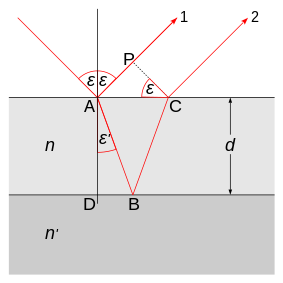
\includegraphics[width=0.7\textwidth]{duenneschicht}
	\caption{Reflexion und Brechung an einer doppelreflektierenden, dünnen Schicht}
	\label{fig:duenneschicht}
\end{figure}

Abbildung \ref{fig:duenneschicht} zeigt eine generelle Prinzipskizze einer dünnen Schicht und beherbergt die drei Variablen $n_1$, $n_2$ und $n_3$ als Brechzahlen, wobei im Folgenden für das Medium $n_1$ Luft angenommen wird, also $n_1=0$ gilt. Die anderen Indices sind größer als $n_1$.

Zwischen den beiden reflektierten Strahlen $a$ und $b$ herrscht ein Gangunterschied $\delta = \overline{AR} + \overline{RB}$, da $b$ einen längeren Weg zurücklegt. Die Strahlen sind zwar in der Skizze parallel, werden sich aber in der Realität nach einer gewissen Strecke trotzdem überlagern, beispielsweise durch Materialunebenheiten. Außerdem ist es ebenfalls wahrscheinlich, dass direkt neben dem Strahl, im Punkt $B$ ein zum Strahl $a$ kohärenter Lichtstrahl auftrifft und reflektiert und auf diese Art sich mit $b$ überlagert.

Es werden destruktive Interferenzen in der Reflexion ausgebildet, wenn für die Schichtdicke bestimmte Bedingungen gelten. Diese Interferenzbedingungen sind abhängig von dem Aufbau der Schichten, da bei der Reflexion von Wellen (Siehe: \referenz{subsec:Reflexion}) Phasensprünge auftreten können.

Bei Licht ist die Regel, dass der Phasensprung um $\pi = \frac{\lambda}{2}$ bei der Reflexion auftritt, wenn an einem optisch dichteren Medium, also an einem Medium mit höherer Brechzahl, reflektiert wird. Wenn an einem Medium mit geringerer Brechzahl reflektiert wird, tritt kein Phasensprung auf. Bei Brechung tritt generell nie ein Phasensprung auf.

Nun wird zudem angenommen, dass der zu betrachtende Lichtstrahl unter einem Winkel $\alpha$ einfällt, so klein, dass die Längen der Strecken $\overline{AR}$ und $\overline{RB}$ gemäß der Kleinwinkelnäherung \glqq in guter Näherung\grqq{} identisch mit der Schichtdicke $d$ sind.

\subsubsection{Fall 1: $n_2 < n_3$}

\noindent Mit der generellen Interferenzbedingung für destruktive Interferenz $\delta = \lambda \cdot (k - \frac{1}{2})$ (Siehe: \gleichungsreferenz{eq:des_interferenz}) und den besprochenen Näherungen gilt bei Phasensprüngen an beiden Schichtübergängen:

\begin{align}
\begin{split}
	\delta &= \lambda_2 \cdot k - \frac{\lambda_2}{2} \quad \text{wobei} \ k \in 1,2,3... \\
\end{split}
\end{align}

\noindent Zu beachten ist hierbei, dass $\lambda_2$ die Wellenlänge im Medium $n_2$ ist. Meistens ist aber die Wellenlänge in Luft angegeben ($\lambda_1$). Aus der \gleichungsreferenz{eq:wellenlaengenaenderung} für die Wellenlänge eines gebrochenen Lichtstrahls ergibt sich für $\lambda_2$ mit $n_1 = 1$:

\begin{align}
\begin{split}
	\frac{\lambda_1}{\lambda_2} &= \frac{n_2}{n_1} \\
	\lambda_2 &= \frac{\lambda_1}{n_2}
\end{split}
\end{align}

\noindent Dann noch $\delta=2d$ aus der Winkelnäherung anwenden und es folgt die Gesamtgleichung für den Fall des Phasensprungs bei beiden Reflexionen ($n_2 < n_3$):

\begin{align}	\label{eq:duenneschichtfall1}
\begin{split}
	2d &= \delta \\
	2d &= \lambda_2 \cdot k - \frac{\lambda_2}{2} \\
	2d &= \frac{\lambda_1 \cdot k}{n_2} - \frac{\lambda_1}{2n_2} \\
	d  &= \frac{\lambda_1 \cdot k}{2n_2} - \frac{\lambda_1}{4n_2} \quad \text{wobei} \ k \in 1,2,3...
\end{split}
\end{align}

\noindent Für den Spezialfall $k=1$ ergibt sich die häufig zitierte Formel:

\begin{align}	\label{eq:duenneschichtfall1spezial}
\begin{split}
	d  &= \frac{\lambda_1}{4n_2}
\end{split}
\end{align}


\subsubsection{Fall 2: $n_2 > n_3$}

\noindent Da der Phasensprung bei der Reflexion am Medium $n_3$ ausgelassen wird, ergibt sich von Natur aus ein Gangunterschied von $\frac{\lambda}{2}$ zwischen den beiden ausfallenden Strahlen, auch wenn die Schicht infinitesimal dünn ist. Daher muss dieses $\frac{\lambda}{2}$ zum Gangunterschied $\delta$ des 1. Falles addiert werden:

\begin{align}
\begin{split}
	\delta_{\text{2.Fall}} &= \delta_{\text{1.Fall}} + \frac{\lambda}{2} \\
	\delta &= \lambda_2 \cdot k - \frac{\lambda_2}{2} + \frac{\lambda_2}{2} \\
	\delta &= \lambda_2 \cdot k \\
	\delta &= \frac{\lambda_1 \cdot k}{n_2} \\
	2d &= \frac{\lambda_1 \cdot k}{n_2} \\
	d &= \frac{\lambda_1 \cdot k}{2n_2} \quad \text{wobei} \ k \in 1,2,3... \\
\end{split}
\end{align}


\subsection{Anwendung}

\subsubsection{Fall 1}

Dieses Prinzip findet Anwendung bei der optischen Vergütung von Linsen in Kameraobjektiven. Da in diesen so wenig Reflexion wie möglich auftreten soll, werden dünne Schichten, deren Brechzahl zwischen Luft und Linse liegt, mit der richtigen Dicke aufgetragen, dass sie bestimmte Wellenlängen, die am häufigsten spiegeln, durch diese destruktive Interferenz auslöschen und so die Intensität des durchgelassenen Lichtes erhöhen und gleichzeitig (un)gewollte Reflexionen auf der Aufnahme\endnote{By Mbhsb.Matthias B. Hullin, Elmar Eisemann, Hans-Peter Seidel, Sungkil Lee: Physically-Based Real-Time Lens Flare Rendering. In: ACM Transactions on Graphics, Vol. 30 (4), 2011 (Proc. SIGGRAPH). - Own work, CC BY-SA 3.0, \$3} vermeiden:

\begin{figure}[H]
	\centering
	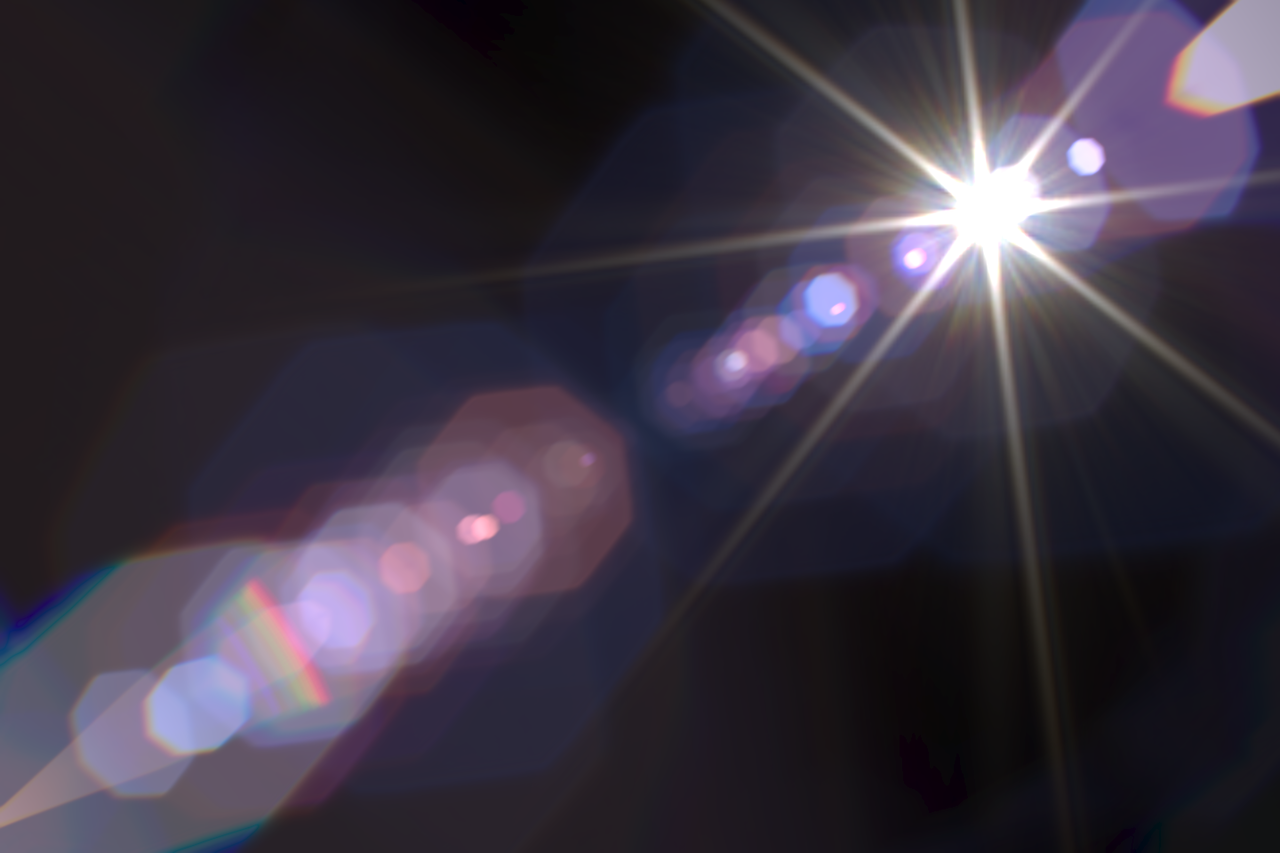
\includegraphics[width=0.7\textwidth]{lens_flare}
	\caption{Reflexe in einer Kameralinse}
\end{figure}

Auch in in öligen Pfützen lässt sich das Phänomen beobachten (Luft - Öl - Wasser: $n_1 < n_2$ und $n_3 > n_2$), man sieht dann verschiedene Farben.

\subsubsection{Fall 2}

Fall 2 tritt in Glimmerplättchen oder Seifenblasen\endnote{„Reflection in a soap bubble edit“ von Brocken Inaglory. The image was edited by user:Alvesgaspar - Eigenes Werk. Lizenziert unter CC BY-SA 3.0 über Wikimedia Commons - \url{https://commons.wikimedia.org/wiki/File:Reflection_in_a_soap_bubble_edit.jpg}} auf (Luft - Seife/Glimmerplättchen - Luft: $n_1 < n_2$ und $n_3 = n_1$):

\begin{figure}[H]
	\centering
	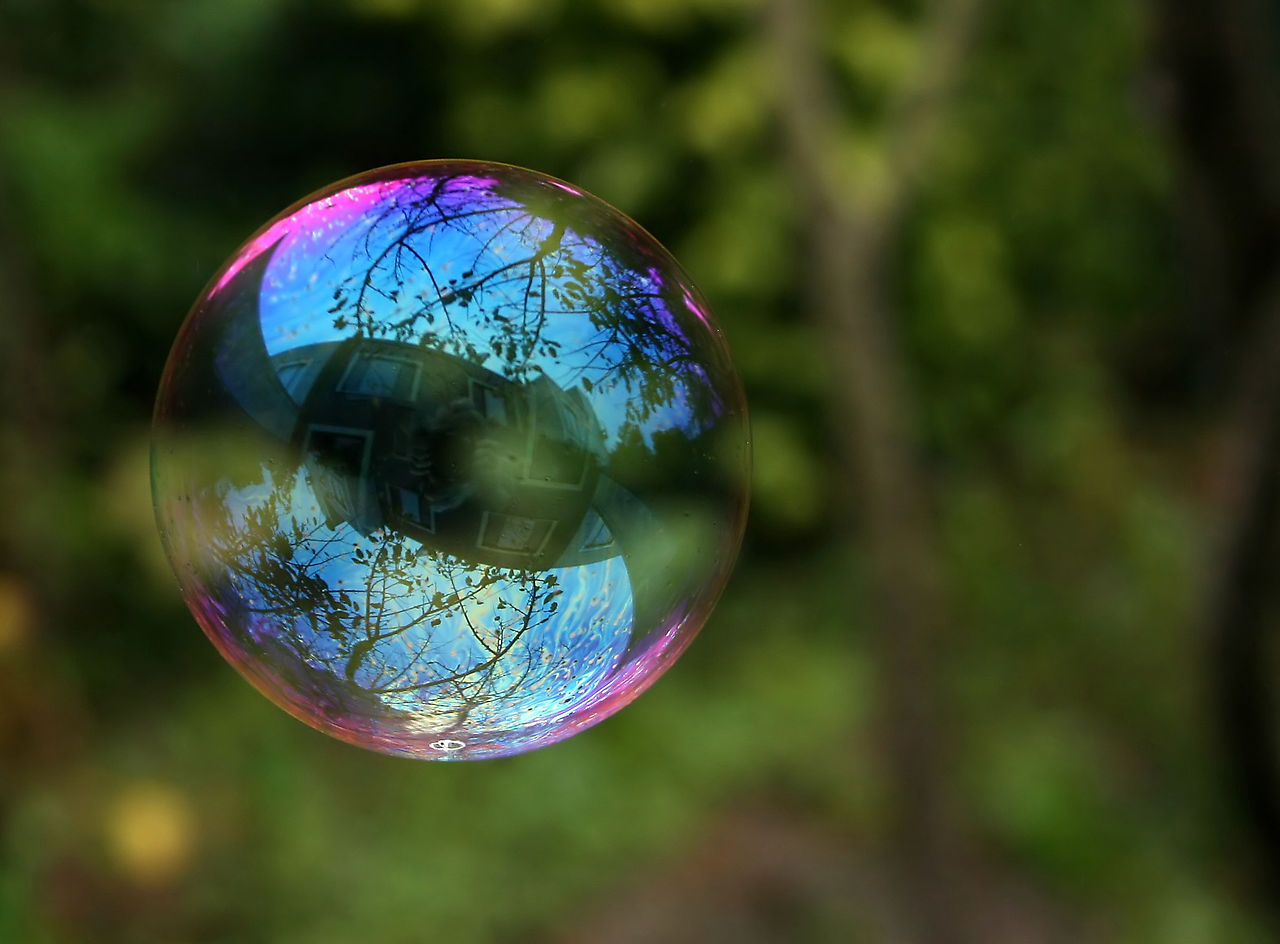
\includegraphics[width=0.7\textwidth]{seifenblase}
	\caption{Interferenz an der Oberfläche einer Seifenblase}
\end{figure}
